\documentclass[conference]{IEEEtran}
\IEEEoverridecommandlockouts
\usepackage[utf8]{inputenc}
%\usepackage[english]{babel}
\usepackage[T1]{fontenc}
% The preceding line is only needed to identify funding in the first footnote. If that is unneeded, please comment it out.
%\usepackage{cite}
\usepackage{amsmath,amssymb,amsfonts}
\usepackage{algorithmic}
\usepackage{graphicx}
\usepackage{textcomp}
\usepackage{xcolor}
\usepackage[backend=biber]{biblatex}
\addbibresource{saltiniai.bib}
\def\BibTeX{{\rm B\kern-.05em{\sc i\kern-.025em b}\kern-.08em
    T\kern-.1667em\lower.7ex\hbox{E}\kern-.125emX}}

\usepackage[labelsep=endash]{caption}
\renewcommand{\figurename}{Figure} \begin{document} \title{Translation of text to images} \author{\IEEEauthorblockN{Teodoras Šaulys} \IEEEauthorblockA{\textit{Institute of informatics} \\ \textit{Faculty of mathematics and informatics}\\ Vilnius, Lithuania \\ teodoras.saulys@mif.stud.vu.lt} \and \IEEEauthorblockN{Povilas Slivinskas} \IEEEauthorblockA{\textit{Institute of informatics} \\ \textit{Faculty of mathematics and informatics}\\ Vilnius, Lithuania \\
povilas.slivinskas@mif.stud.vu.lt}
}
\maketitle

\begin{abstract}
In this paper we analyze the performance of Stable Diffusion, fine-tuned using different techiques using a Pokemon dataset \cite{pinkney2022pokemon}. The primary focus of this team project is to thoroughly analyze the performance of Stable Diffusion and assess its ability to be fine-tuned effectively with the same dataset and parameters, particularly in generating images based on textual descriptions. By utilizing pre-trained model on the selected dataset, we compare the results and delve into the field of fine-tuning text-to-image models.
\end{abstract}

\begin{IEEEkeywords}
fine-tuning, text-to-image, diffusion models, large language models, weight freezing, LoRA
\end{IEEEkeywords}

\section{Introduction}
Text-to-image synthesis has gained significant attention in recent years due to its potential applications in various domains such as computer vision, creative arts, and multimedia content generation. The ability to generate realistic images from textual descriptions opens up new possibilities for content creation, storytelling, and even assisting individuals with limited artistic skills to visualize their ideas. In this paper, we delve into the realm of fine-tuning text-to-image models, focusing on Stable Diffusion, using the Pokemon dataset \cite{pinkney2022pokemon}. Our objective is to explore the effectiveness of fine-tuning Stable Diffusion with the same dataset and parameters, but with different fine-tuning techniques. We are aiming to enhance the model's capability to generate visually coherent and accurate images. Through a comprehensive analysis of the performance and results, we aim to provide insights into the potential of fine-tuning text-to-image models and contribute to the advancement of this exciting field.

\section{Dataset}
The dataset used in this paper \cite{pinkney2022pokemon} consists of 838 image-description pairs of Pokémons. The description for each Pokémon was generated with the Bootstrapping Language-Image Pre-training (BLIP) framework, which means that the descriptions may not be perfect and may have some inaccuracies. However, for our purposes this should not be a big hindrance.

\section{Model used}
For this paper we used Stable Diffusion, following the guidelines in \cite{patil2022stable} in order to get it running. The model is based on a type of a diffusion model, which is called Latent Diffusion, which is proposed and explored in \cite{diffus}. The basic principle of such machine learning models is that they employ a step-by-step denoising of random Gaussian noise to create images.

\begin{figure}
\centerline{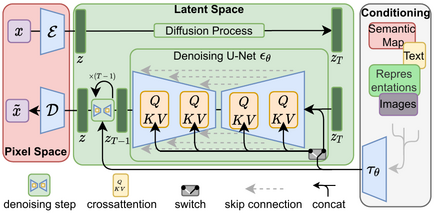
\includegraphics[scale=1.8]{diff.png}}
\caption{Inner workings of Stable Diffusion}
\label{fig}
\end{figure}

\section{Methods}

\subsection{Classic fine-tuning}
Fine-tuning text-to-image models involves the process of adapting pre-trained models, originally trained on a large dataset, to generate visually coherent and accurate images based on textual descriptions. By fine-tuning these models with a specific dataset and parameters, we aim to enhance their ability to generate images that align with the given textual input. Fine-tuning leverages the pre-existing knowledge and learned features of the models, allowing them to specialize and generate more contextually relevant images in response to textual prompts. This process facilitates the transfer of knowledge from the pre-trained models to the target task, enabling improved performance and generating visually compelling images that effectively capture the essence of the provided textual descriptions.

\subsection{Fine-tuning parameters}
For fine-tuning both the StableDiffusion and <insert model> text-to-image models, we employed a consistent set of parameters. The following list provides a brief explanation of each parameter:\begin{itemize}
\item{Dataset name: lambdalabs/pokemon-blip-captions - a dataset containing used for training that contains Pokemon-related image-caption pairs.}
\item{Use\_ema: true - Enables the use of Exponential Moving Average (EMA) during training, which can stabilize the model's performance.}
\item{Resolution: 512 - sets the resolution of the generated images to 512x512 pixels, ensuring a consistent output size.}
\item{Center\_crop: true - Applies center cropping to the input images, focusing on the central region for training.}
\item{Random\_flip: true - Randomly flips the images horizontally, introducing additional diversity during training.}
\item{Train\_batch\_size: 4 - Specifies the batch size for training, determining the number of samples processed in each training iteration.}
\item{Gradient\_accumulation\_steps: 4 - accumulates gradients over multiple steps, effectively increasing the effective batch size and - allowing for more stable training.}
\item{Gradient\_checkpointing: true - saving memory by trading off computational efficiency for memory consumption during backpropagation.}
\item{Max\_train\_steps: 100 - limits the maximum number of training steps to 100, controlling the duration of the training process.}
\item{Learning\_rate: 1e-05 - sets the initial learning, governing the step size for adjusting the model's parameters during training.}
\item{Max\_grad\_norm: 1 - Specifies the maximum gradient norm value, which is used for gradient clipping to prevent exploding gradients.}
\item{LR\_scheduler: Constant - sets the learning rate scheduler to "constant," indicating a fixed learning rate throughout the training process.}
\end{itemize}

By utilizing these parameters consistently for both models, we aim to ensure a fair comparison and evaluate the effectiveness of fine-tuning in generating images based on textual descriptions from the chosen Pokemon dataset.

\subsection{Fine-tuning with Low-Rank Adaptation of Large Language Models (LoRA)}
Low-Rank adaptation of large language models was proposed by researchers from Microsoft as a viable fine-tuning technique for large language models \cite{hu2021lora}. The main problem of fine-tuning such models with numerous parameters is that it is often expensive and time-consuming, because all of the parameters are involved during fine-tuning. Instead an alternative is proposed, which consists of freezing the pre-trained weights and injecting trainable rank decomposition matrices into transformer's layers. As a result, instead of training the model's weights, the weights of the injected layers are trained. Originally LoRA was intended for large language models, nevertheless it is applicable to diffusion models, in our specific case Stable Diffusion. In our instance, LoRA can be used in the cross-attention layers, which are involved in mapping image representations with the given prompts. The main advantages of such fine-tuning approach are as follows:
\begin{itemize}
\item Significantly faster training
\item The resulting weights are much smaller
\item Computing resources required for this approach are more modest
\end{itemize}

Above mentioned points greatly increase availability to fine-tuning Stable Diffusion to a wider population of users which may not have the bleeding-edge hardware.

%\begin{equation}
%\mathcal{L}({\bf X}, {\bf Y}) = \frac{1}{w \cdot h} \sum_{i=1}^h \sum_{j=1}^w (X_{i, j} - Y_{i, j})^2
%\label{eq:lygtis1}
%\end{equation}

%Taikyta nuostolių funkcija ~\eqref{eq:lygtis1}.

%\begin{align}
%y & = f(x) \nonumber \\
%%f & = f_1(f_2(x))
%\label{eq:lygtis2}
%\end{align}

%Taikytas modelis ~\eqref{eq:lygtis2}.

%\subsection{Equations}

%\subsection{Paveikslėliai ir lentelės}

%\begin{table}[htbp]
%\caption{Lentelės aprašas}
%\begin{center}
%\begin{tabular}{|c|c|c|c|}
%\hline
%a & b & c &  d \\
%\hline
%\end{tabular}
%\label{tab1}
%\end{center}
%\end{table}

\section{Results}

%\bibliographystyle{plain}
%\bibliography{saltiniai}
\printbibliography[heading=bibintoc]

\end{document}
